\section{Resultados}
\label{resultados}


Os requisitos foram separados e divididos pelos requisitos através dos códigos \textit{r1} a \textit{r4}. Para o código \textit{r1}, obteve-se simplesmente uma interface do usuário em que com dois cliques do mouse era possível medir a distância em píxeis entre dois pontos.

Com a captura das imagens pelo algoritmo \textit{get\_images}, obteve-se a média e desvio padrão das 5 matrizes intrínsecas e coefientes de distorção através do algoritmo \textit{r2}. Os valores dos parâmetros das matrizes intrínsecas são mostrados pela Tabela (\ref{tab:intrisec}). 

\begin{table}[!ht]
\centering
\label{tab:intrisec}
\caption{Parâmetros intrínsecos da matriz $In$ para diferentes posições a uma distância de 75 cm do plano da câmera}
\begin{tabular}{c|c|c|c|c|c|c|}
\cline{2-7}
                            & $In_1$ & $In_2$ & $In_3$ & $In_4$ & $In_5$ & $In\ (\overline{x} \pm \sigma)$           \\ \hline
\multicolumn{1}{|c|}{$f_x$} & 721    & 1154   & 1739   & 1052   & 1955   & $1324 \pm 455$ \\ \hline
\multicolumn{1}{|c|}{$f_y$} & 728    & 1164   & 1846   & 1079   & 3219   & $1607 \pm 884$ \\ \hline
\multicolumn{1}{|c|}{$c_x$} & 634    & 714    & 639    & 649    & 633    & $654 \pm 30$   \\ \hline
\multicolumn{1}{|c|}{$c_y$} & 374    & 316    & 369    & 334    & 353    & $349 \pm 22$   \\ \hline
\end{tabular}
\end{table}


\begin{figure}[!ht]
\caption{Posições das fotos tiradas do tabuleiro}
\end{figure}
\begin{minipage}{0.3\textwidth}
\centering
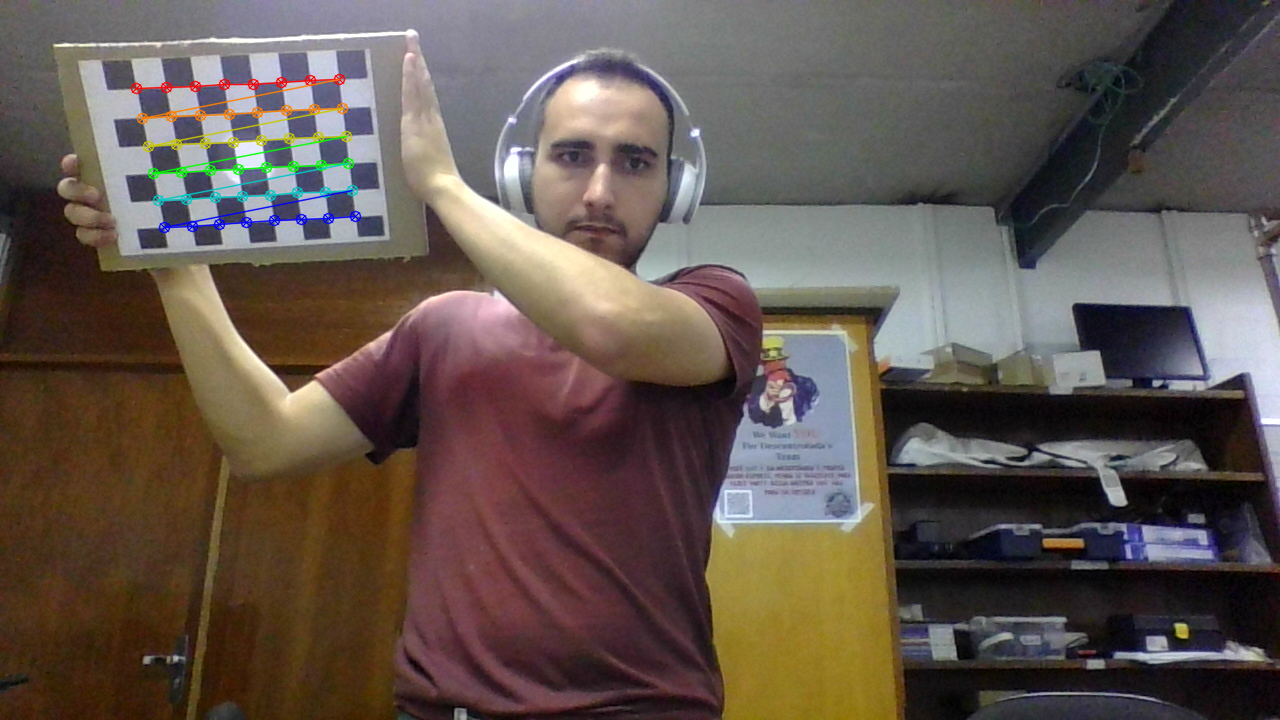
\includegraphics[width = \textwidth]{img/2.png}
\end{minipage}
\begin{minipage}{0.3\textwidth}
\centering
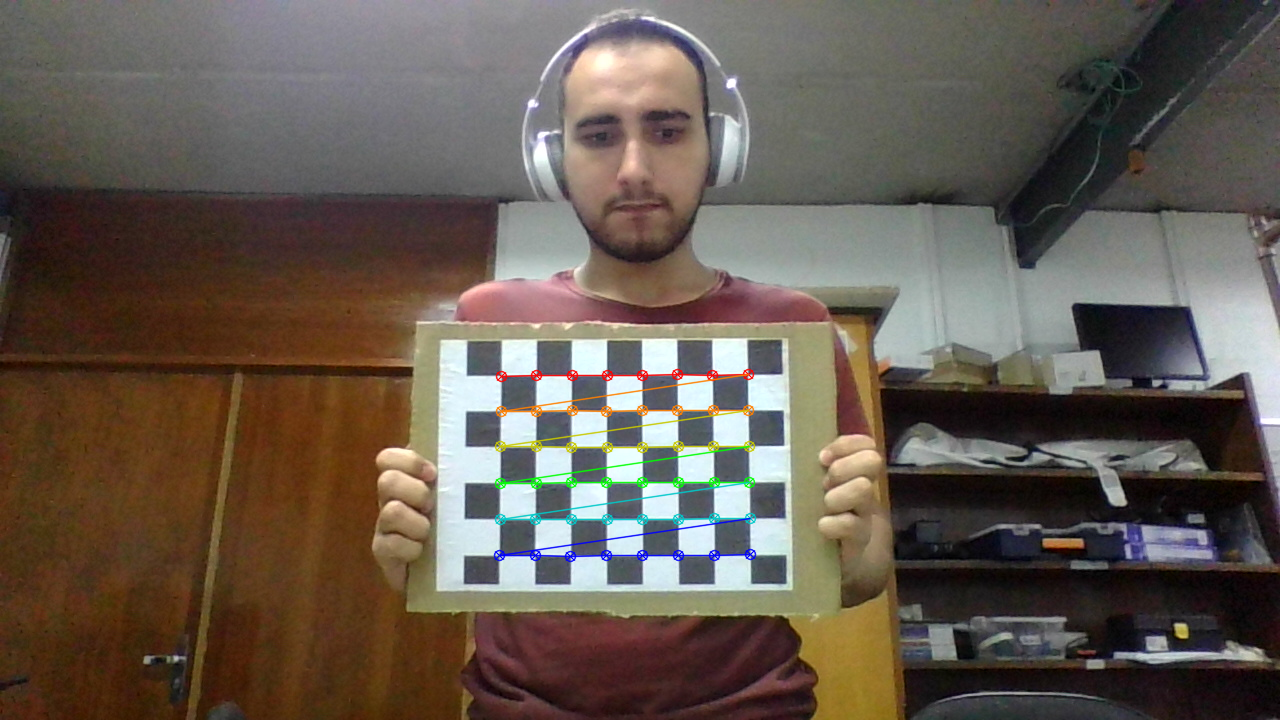
\includegraphics[width = \textwidth]{img/1.png}
\end{minipage}
\begin{minipage}{0.3\textwidth}
\centering
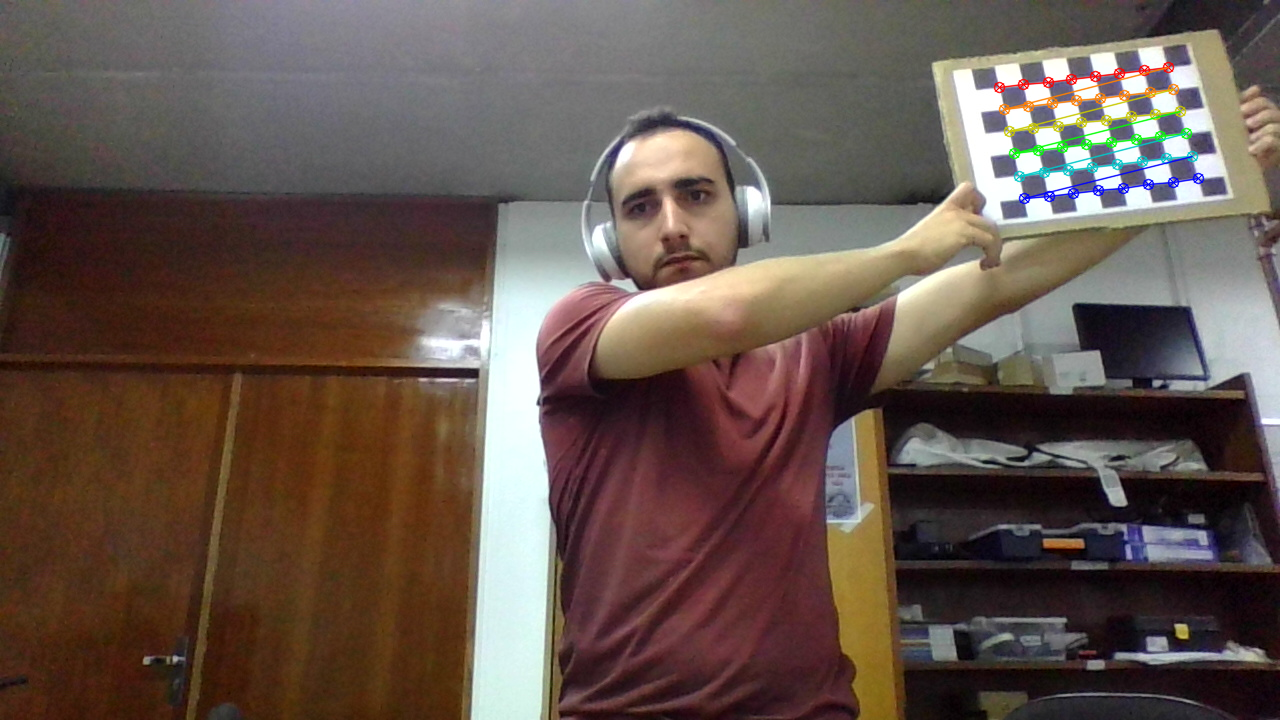
\includegraphics[width = \textwidth]{img/3.png}
\end{minipage}

\begin{minipage}{0.5\textwidth}
\begin{flushright}
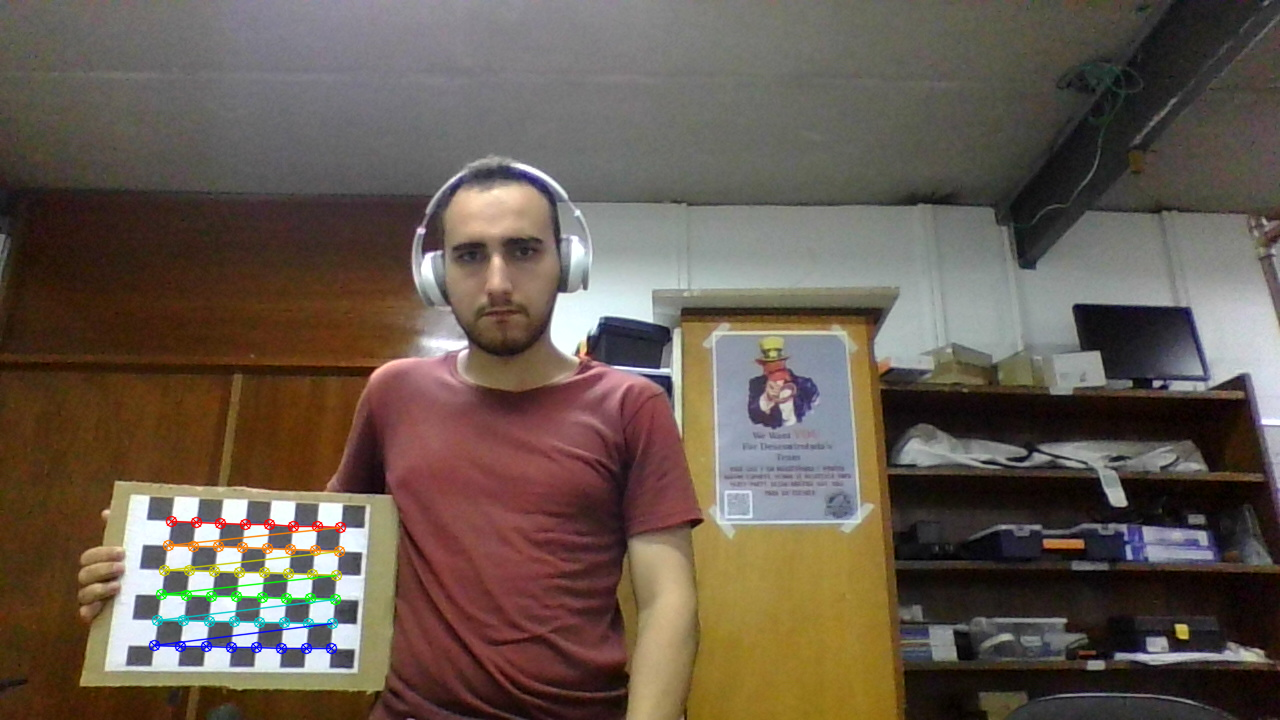
\includegraphics[width = 0.6\textwidth]{img/4.png}
\end{flushright}
\end{minipage}
\begin{minipage}{0.5\textwidth}
\begin{flushleft}
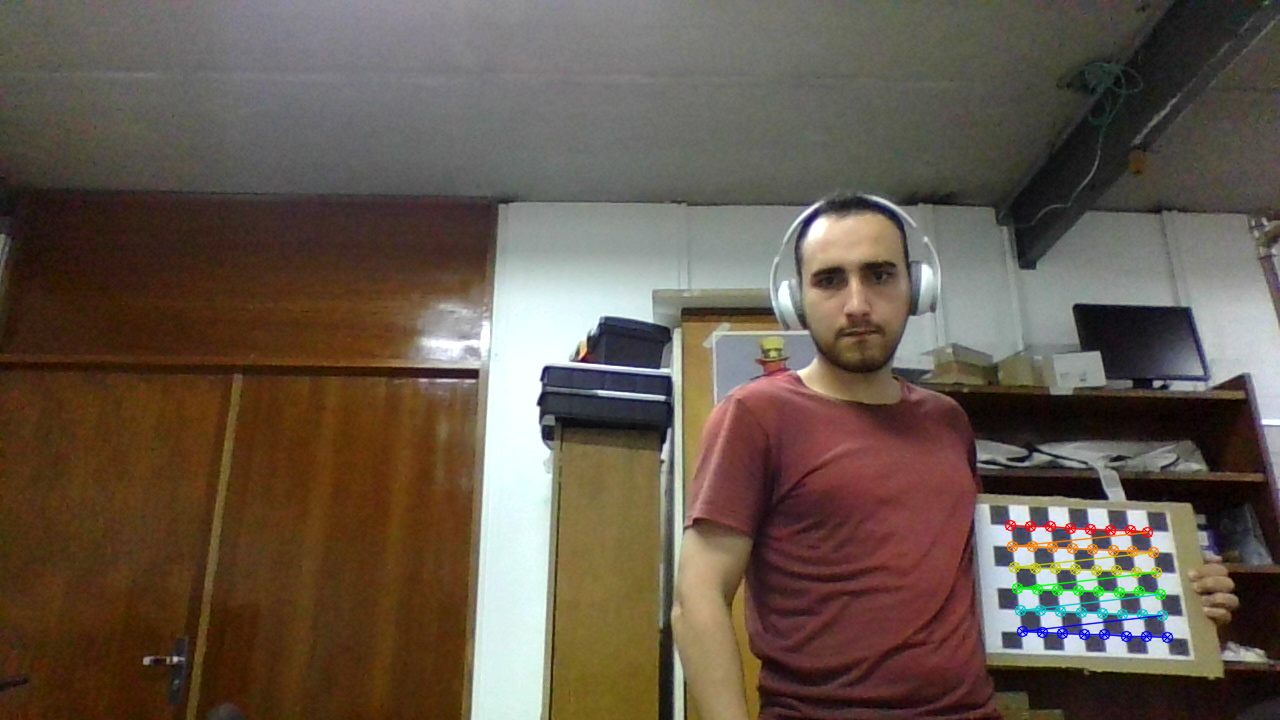
\includegraphics[width = 0.6\textwidth]{img/5.png}
\end{flushleft}
\end{minipage}

Uma vez que tenha-se os parâmetros intrínsecos obtidos, fazendo os procedimentos descritos na metodologia pôde-se estimar os valores dos parâmetros extrinsecos. Utilizando os vetores fornecidos pela função \textit{calibrateCamera}, e calculado a média com os 25 valores para cada uma das 3 distâncias, obtemos a Tabela (\ref{tab:extrinsec}). Os valores das incertezas dos vetores foram todos menores que $5\%$.

\begin{table}[!ht]
\centering
\label{tab:extrinsec}
\caption{Parâmetros extrínsecos da matriz $Ex$ para diferentes distâncias no eixo focal}
\begin{tabular}{c|c|c|c|c|c|c|}
% \cline{2-7}
%                              & $rot_1$            & $rot_2$           & $rot_3$            & $tra_1$          & $tra_2$          & $tra_3$          \\ \hline
% \multicolumn{1}{|c|}{35 cm}  & $-0.190 \pm 0.004$ & $0.06 \pm 0.01$   & $0.001 \pm 0.005$  & $-2.61 \pm 0.03$ & $-2.33 \pm 0.02$ & $11.78 \pm 0.06$ \\ \hline
% \multicolumn{1}{|c|}{70 cm}  & $-0.31 \pm 0.02$   & $0.23 \pm 0.01$   & $-0.016 \pm 0.006$ & $2.89 \pm 0.03$  & $0.70 \pm 0.04$  & $33.40 \pm 0.07$ \\ \hline
% \multicolumn{1}{|c|}{120 cm} & $-0.45 \pm 0.02$   & $0.017 \pm 0.005$ & $-0.021 \pm 0.001$ & $-1.10 \pm 0.04$ & $10.89 \pm 0.04$ & $75.5 \pm 0.3$   \\ \hline
\cline{2-7}
                             & \multicolumn{3}{c|}{Vetor Rotação} & \multicolumn{3}{c|}{Vetor Translação} \\ \hline
\multicolumn{1}{|c|}{35 cm}  & $-0.190$   & $0.06$    & $0.001$   & $-2.61$     & $-2.33$    & $11.78$    \\ \hline
\multicolumn{1}{|c|}{75 cm}  & $-0.31$    & $0.23$    & $-0.016$  & $2.89$      & $0.70$     & $33.40$    \\ \hline
\multicolumn{1}{|c|}{120 cm} & $-0.45$    & $0.017$   & $-0.021$  & $-1.10$     & $10.89$    & $75.5$     \\ \hline
\end{tabular}
\end{table}

Uma vez obtidos os vetores médios, precisou-se apenas da matriz $R$ responsável pela rotação. Para obtenção dela a partir do vetor de rotação, utilizou-se a função \textit{Rodrigues} da OpenCV. Com a matriz $R$ e o vetor de translação, bastou montar a matriz que transforma as coordenadas do mundo tridimensional(em coordenadas homogêneas) para as coordenadas em pixeis segundo a Equação (\ref{eq:matrizes}). Para a distância de $75$ cm, tem-se a matriz extrínseca mostrada na Equação (\ref{eq:MatrizExtrinseca})

\begin{equation}
\label{eq:MatrizExtrinseca}
\left[R  | t \right] = 
\begin{bmatrix}
-0.9733 & -0.0195 & 0.2286 & 2.8870 \\
-0.0517 &  0.9521 & 0.3015 & 0.7016 \\
-0.2236 & -0.3053 & 0.9257 & 33.405 
\end{bmatrix}
\end{equation}

Após obtenção da matriz extrinseca, tentou-se aplicar para cumprir o requisito 4. Mas das 15 tentativas de calibração realizadas, a imagem ficava mais distorcida que o normal, ou seja, mais distorcida que não aplicar qualquer correção. As grandes deformações nas laterais apareciam durante a calibração dos valores intrínsecos indicando um erro na calibração dos valores intrínsecos. E a movimentação para baixo do centro da imagem, como mostra a Figura (\ref{fig:distorcao}), indica que há um erro também na calibração dos valores extrínsecos.

\begin{figure}[!ht]
\centering
\label{fig:distorcao}
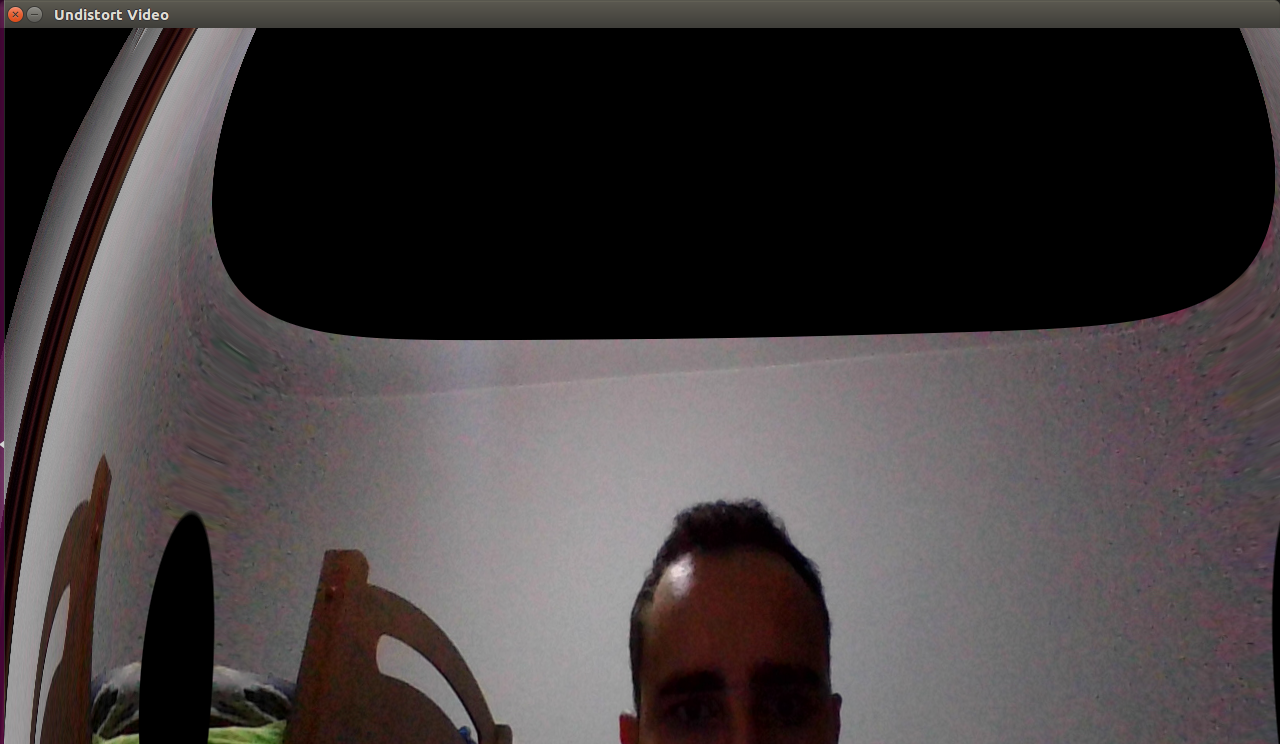
\includegraphics[width=0.5\textwidth]{img/distorcao.png}
\caption{Produto final após a correção dos valores intrínsecos e extrínsecos}
\end{figure}